\documentclass{article}

% packages
\usepackage{amsmath, amsthm, thmtools, amsfonts, amssymb, luacode, catchfile, tikzducks, hyperref, ifthen}
\ifcsname c@kobocompile\endcsname
	\usepackage[a5paper, total={1072pt, 1448pt}, margin=10pt, includeheadfoot]{geometry} % set page margins
\else
	\usepackage[a4paper, margin=50pt, includeheadfoot]{geometry}
\fi
\usepackage[shortlabels]{enumitem}
\usepackage[skip=3pt, indent=0pt]{parskip}

% language
\usepackage[bidi=basic, layout=tabular, provide=*]{babel}
\ifcsname c@english\endcsname
	\babelprovide[main, import]{english}
\else
	\babelprovide[main, import]{hebrew}
	\babelprovide{rl}
\fi
%\babelfont{rm}{Libertinus Serif}
\babelfont{rm}[Renderer=Harfbuzz]{Libertinus Serif}
\babelfont{sf}{Libertinus Sans}
\babelfont{tt}{Libertinus Mono}

% style
\AddToHook{cmd/section/before}{\clearpage}	% Add line break before section
\linespread{1.3}
\setcounter{secnumdepth}{0}		% Remove default number tags from sections, this won't do well with theorems
\AtBeginDocument{\setlength{\belowdisplayskip}{3pt}}
\AtBeginDocument{\setlength{\abovedisplayskip}{3pt}}
\graphicspath{ {../images/} }

% operators
\DeclareMathOperator\cis{cis}
\DeclareMathOperator\Sp{Sp}
\DeclareMathOperator\tr{tr}
\DeclareMathOperator\im{Im}
\DeclareMathOperator\re{Re}
\DeclareMathOperator\diag{diag}
\DeclareMathOperator*\lowlim{\underline{lim}}
\DeclareMathOperator*\uplim{\overline{lim}}
\DeclareMathOperator\rng{rng}
\DeclareMathOperator\Sym{Sym}
\DeclareMathOperator\Arg{Arg}
\DeclareMathOperator\Log{Log}
\DeclareMathOperator\dom{dom}
\DeclareMathOperator\supp{Supp}
\DeclareMathOperator\var{Var}
\DeclareMathOperator\cov{Cov}

% commands
%\renewcommand\qedsymbol{\textbf{מש''ל}}
%\renewcommand\qedsymbol{\fbox{\emoji{lizard}}}
\newcommand{\Aa}[0]{\mathcal{A}}
\newcommand{\Bb}[0]{\mathcal{B}}
\newcommand{\CC}[0]{\mathbb{C}}
\newcommand{\Cc}[0]{\mathcal{C}}
\newcommand{\EE}[0]{\mathbb{E}}
\newcommand{\FF}[0]{\mathbb{F}}
\newcommand{\Ff}[0]{\mathcal{F}}
\newcommand{\Ii}[0]{\mathcal{I}}
\newcommand{\Gg}[0]{\mathcal{G}}
\newcommand{\Ll}[0]{\mathcal{L}}
\newcommand{\Mm}[0]{\mathcal{M}}
\newcommand{\NN}[0]{\mathbb{N}}
\newcommand{\Nn}[0]{\mathcal{N}}
\newcommand{\PP}[0]{\mathbb{P}}
\newcommand{\Pp}[0]{\mathcal{P}}
\newcommand{\QQ}[0]{\mathbb{Q}}
\newcommand{\RR}[0]{\mathbb{R}}
\newcommand{\Rr}[0]{\mathcal{R}}
\newcommand{\Ss}[0]{\mathcal{S}}
\newcommand{\TT}[0]{\mathbb{T}}
\newcommand{\Uu}[0]{\mathcal{U}}
\newcommand{\Vv}[0]{\mathcal{V}}
\newcommand{\Ww}[0]{\mathcal{W}}
\newcommand{\ZZ}[0]{\mathbb{Z}}
\newcommand{\acts}[0]{\circlearrowright}
\newcommand{\explain}[2] {
	\begin{flalign*}
		 && \text{#2} && \text{#1}
	\end{flalign*}
}
\newcommand{\maketitleprint}[0]{ \begin{center}
	%\begin{tikzpicture}[scale=3]
	%	\duck[graduate=gray!20!black, tassel=red!70!black]
	%\end{tikzpicture}	
	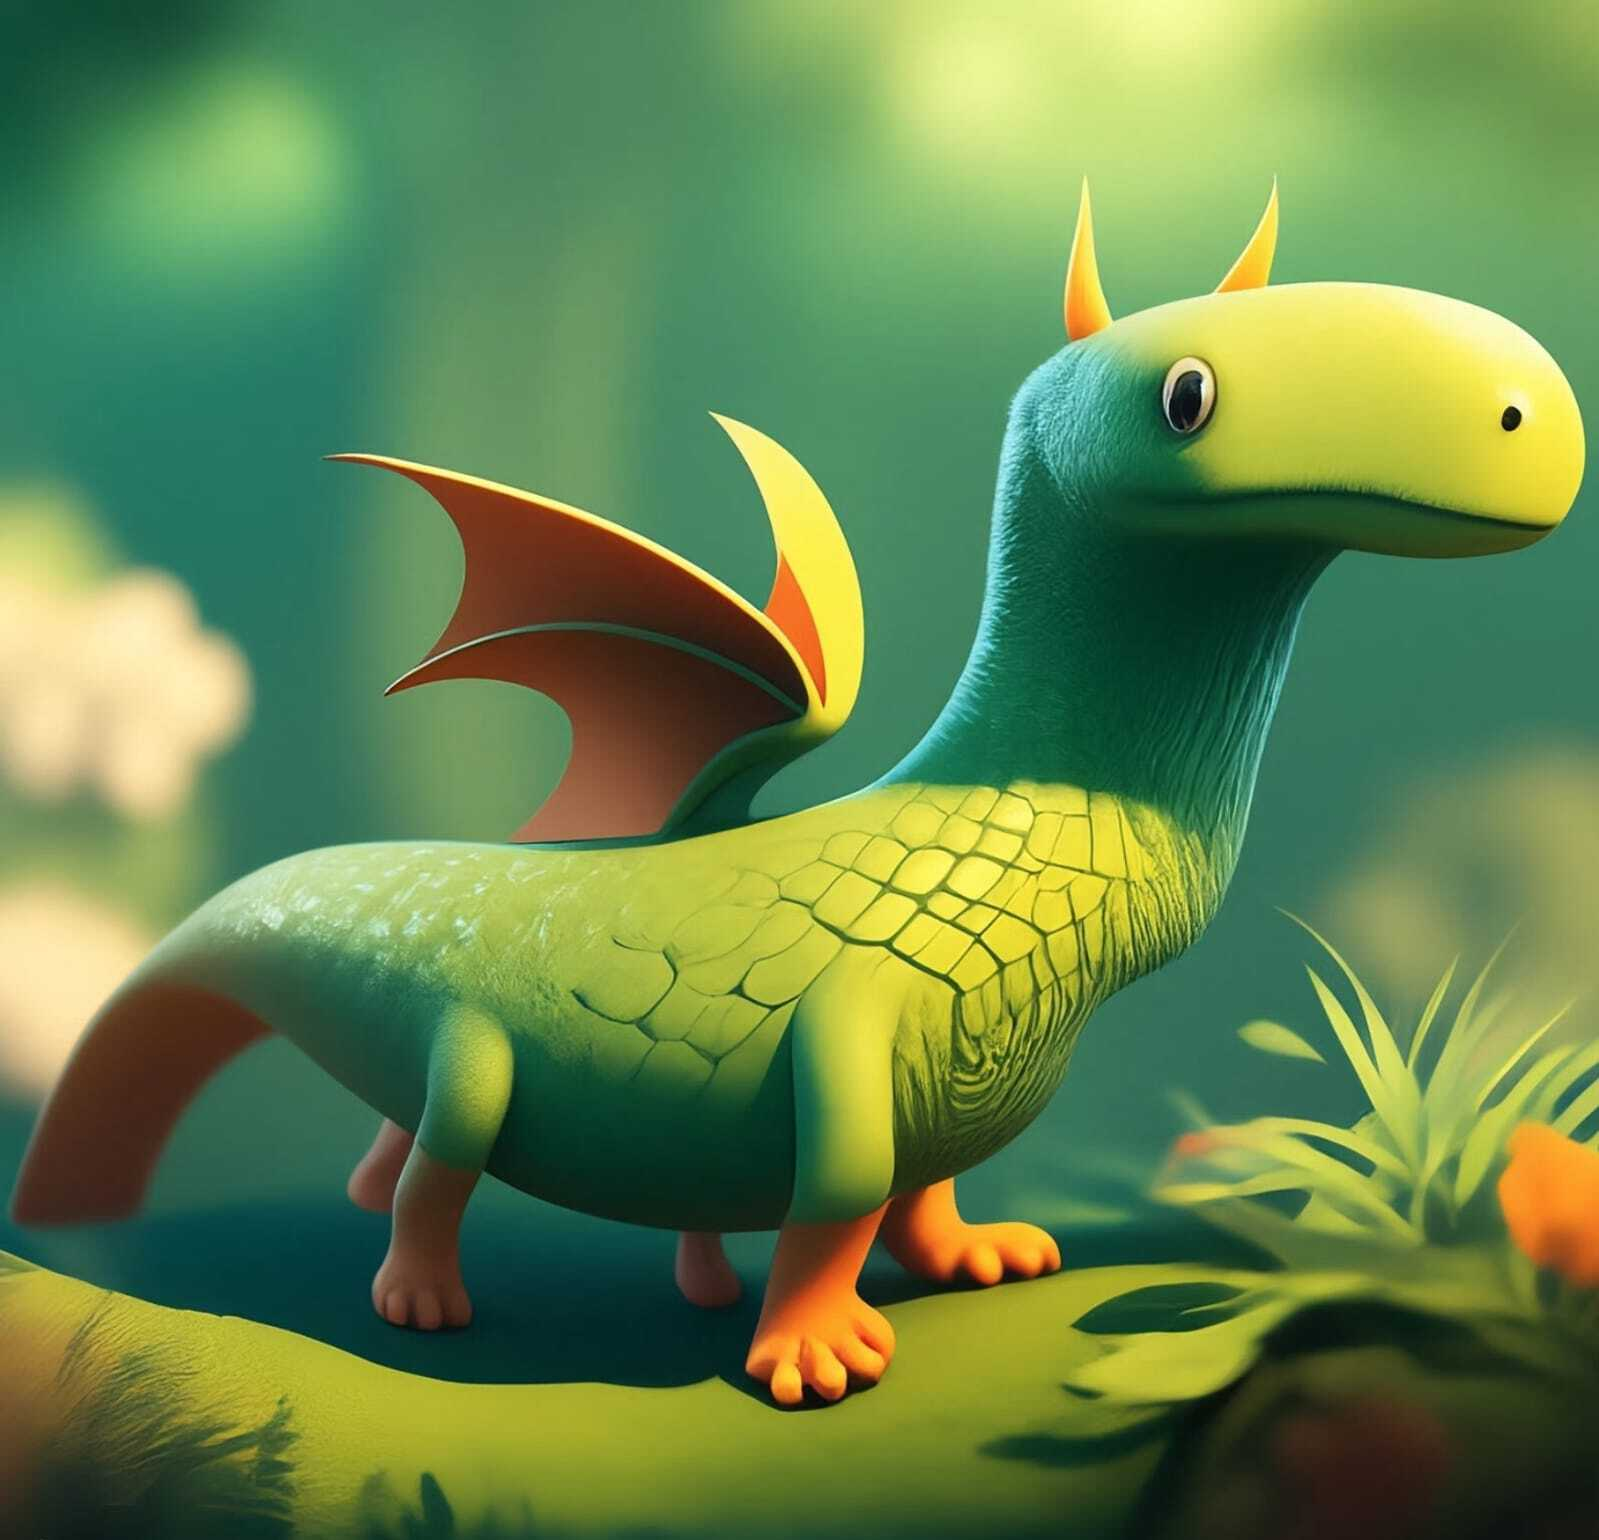
\includegraphics[width=6cm]{cover}
\end{center}
}

% theorem commands
\newtheoremstyle{c_remark}
	{}	% Space above
	{}	% Space below
	{}% Body font
	{}	% Indent amount
	{\bfseries}	% Theorem head font
	{}	% Punctuation after theorem head
	{.5em}	% Space after theorem head
	{\thmname{#1}\thmnumber{ #2}\thmnote{ \normalfont{\text{(#3)}}}}	% head content
\newtheoremstyle{c_definition}
	{3pt}	% Space above
	{3pt}	% Space below
	{}% Body font
	{}	% Indent amount
	{\bfseries}	% Theorem head font
	{}	% Punctuation after theorem head
	{.5em}	% Space after theorem head
	{\thmname{#1}\thmnumber{ #2}\thmnote{ \normalfont{\text{(#3)}}}}	% head content
\newtheoremstyle{c_plain}
	{3pt}	% Space above
	{3pt}	% Space below
	{\itshape}% Body font
	{}	% Indent amount
	{\bfseries}	% Theorem head font
	{}	% Punctuation after theorem head
	{.5em}	% Space after theorem head
	{\thmname{#1}\thmnumber{ #2}\thmnote{ \text{(#3)}}}	% head content

\ifcsname c@english\endcsname
	\theoremstyle{plain}
	\newtheorem{theorem}{Theorem}[section]
	\newtheorem{lemma}[theorem]{Lemma}
	\newtheorem{proposition}[theorem]{Proposition}
	\newtheorem*{proposition*}{Proposition}
	%\newtheorem{corollary}[theorem]{אין חלופה עברית}

	\theoremstyle{definition}
	\newtheorem{definition}[theorem]{Definition}
	\newtheorem*{definition*}{Definition}
	\newtheorem{example}{Example}[section]
	\newtheorem{exercise}{Exercise}[section]

	\theoremstyle{remark}
	\newtheorem*{remark}{Remark}
	\newtheorem*{solution}{Solution}
	\newtheorem{conclusion}[theorem]{Conclusion}
	\newtheorem{notation}[theorem]{Notation}
\else
	\theoremstyle{c_plain}
	\newtheorem{theorem}{משפט}[section]
	\newtheorem{lemma}[theorem]{למה}
	\newtheorem{proposition}[theorem]{טענה}
	\newtheorem*{proposition*}{טענה}
	%\newtheorem{corollary}[theorem]{אין חלופה עברית}

	\theoremstyle{c_definition}
	\newtheorem{definition}[theorem]{הגדרה}
	\newtheorem*{definition*}{הגדרה}
	\newtheorem{example}{דוגמה}[section]
	\newtheorem{exercise}{תרגיל}[section]

	\theoremstyle{c_remark}
	\newtheorem*{remark}{הערה}
	\newtheorem*{solution}{פתרון}
	\newtheorem{conclusion}[theorem]{מסקנה}
	\newtheorem{notation}[theorem]{סימון}
\fi

% Questions related commands
\newcounter{question}
\setcounter{question}{1}
\newcounter{sub_question}
\setcounter{sub_question}{1}

\ifcsname c@english\endcsname
	\newcommand{\question}[1][0]{
		\ifthenelse{#1 = 0}{}{\setcounter{question}{#1}}
		\section{Question \arabic{question}}
		\addtocounter{question}{1}
		\setcounter{sub_question}{1}
	}

	\newcommand{\subquestion}[1][0]{
		\ifthenelse{#1 = 0}{}{\setcounter{sub_question}{#1}}
		\subsection{Part \alph{sub_question}}
		\addtocounter{sub_question}{1}
	}
\else
	\newcommand{\question}[1][0]{
		\ifthenelse{#1 = 0}{}{\setcounter{question}{#1}}
		\section{שאלה \arabic{question}}
		\addtocounter{question}{1}
		\setcounter{sub_question}{1}
	}

	\newcommand{\subquestion}[1][0]{
		\ifthenelse{#1 = 0}{}{\setcounter{sub_question}{#1}}
		\subsection{סעיף \localecounter{letters.gershayim}{sub_question}}
		\addtocounter{sub_question}{1}
	}
\fi

% import lua and start of document
\directlua{common = require ('../common')}

\GetEnv{AUTHOR}

% headers
\author{\AUTHOR}
\date\today

\title{פתרון מטלה 07 --- מבנים אלגבריים 1 (80445)}

\begin{document}
\maketitle
\maketitleprint{}

\Question{}
\Subquestion{}
נוכיח כי חבורה מסדר 45 היא לא פשוטה.
\begin{proof}
	נבחן את $Syl_5(G)$ עבור $G$ כלשהי המקיימת $|G| = 45$. \\*
	ממשפט סילו השלישי נקבל כי $n_5 = 1 (\mod 5)$ ולכן נסיק $n_5 = 1, 6, 26$ ואלה האופציות היחידות מטעמי גודל החבורה. \\*
	אנו גם יודעים כי $n_5 \mid 9$ ולכן $n_5 = 1$ בלבד וממשפט סילו השני נוכל להסיק כי קיימת תת־חבורה נורמלית מסדר $5$ ובהתאם $G$ לא פשוטה.
\end{proof}

\Subquestion{}
נוכיח כי אם חבורה מסדר 30 אז היא לא פשוטה.
\begin{proof}
	תהי $G$ חבורה כך ש־$|G| = 30 = 2 \cdot 3 \cdot 5$. \\*
	ממשפטי סילו הראשון והשלישי נסיק כי $n_3 = 1, 10$. אם $n_3 = 1$ ממשפט סילו השני נסיק כי $G$ לא פשוטה ולכן נניח כי $n_3 = 10$. \\*
	נגדיר $\{ P_1, \dots, P_{10} \} = Syl_3(G)$ ונסיק כי $P_i \simeq \ZZ_{/3}$ לכל $i \in [10]$ ולכן גם לכל $i \ne j \in [10]$ נקבל $P_i \cap P_j = \{ e \}$. \\*
	נסיק אם כן כי קיימים $20$ איברים מסדר $3$ ב־$G$.

	באופן דומה נקבל כי $n_5 = 1, 6$ ולכן נניח כי $n_5 = 6$ בלבד, ונקבל כי ישנן שש חבורות מסדר 5 ולכן ישנם $25$ איברים מסדר $5$ בסתירה למה שמצאנו זה עתה, ולכן או $n_5 = 1$ או $n_3 = 1$ ובכל מקרה $G$ לא פשוטה.
\end{proof}

\Question{}
תהי $G$ חבורה מסדר סופי ו־$p$ ראשוני.

\Subquestion{}
נוכיח כי כל תת־חבורת־$p$ שנסמן $Q \le G$ מוכלת בחבורת $p$־סילו של $G$.
\begin{proof}
	מלמה שהוכחה בהרצאה נסיק כי קיים $g \in G$ כך ש־$g Q g^{-1} \le P$ כאשר $P$ תת־חבורה $p$־סילו של $G$. \\*
	אנו יודעים ממשפט סילו השני כי כל חבורות $p$־סילו צמודות, ולכן גם $g^{-1}$ מצמיד את $P$ ל־$P'$ חבורה $p$־סילו כלשהי, ונקבל
	\[
		g^{-1}g Q g^{-1}g = Q \le g^{-1} P g = P'
	\]
\end{proof}

\Subquestion{}
תהי $H \le G$ תת־חבורה. נוכיח כי כל תת־חבורה $p$־סילו $P_H \le H$ מוכלת בתת־חבורת $p$־סילו $P_G \le G$.
\begin{proof}
	$P_H$ היא חבורת $p$ על־פי הגדרה וכמובן $P_H \le H \le G \implies P_H \le G$ ולכן תנאי הסעיף הקודמים מתקיימים ונובע כי $P_H$ מוכלת באיזושהי חבורה $p$־סילו $P_G \le G$.
\end{proof}

\Subquestion{}
תהי $N \triangleleft G$ תת־חבורה נורמלית. נוכיח כי לכל חבורת $p$־סילו $P \le G$, החבורה $P \cap N$ היא תת־חבורה $p$־סילו של $N$ ו־$PN/N$ היא תת־חבורה $p$־סילו של $G/N$.
\begin{proof}
	אנו יודעים כי $N$ היא איחוד של מחלקות צמידות של $G$, ואנו יודעים גם כי ל־$G$ מחלקות צמידות של תת־חבורות $p$־סילו של $G$. \\*
	אילו $N$ מורכבת ממחלקת הצמידות של $P$ אז בהתאם $P = P \cap N$, ולכן חיתוך זה הוא חבורת $p$, וחבורת $p$־סילו של $G$, ולכן משיקולי גודל בוודאי שגם תת־חבורת $p$־סילו של $N$. \\*
	נניח אם כן כי $N$ לא מורכבת ממחלקת הצמידות של $P$, ןלכן כמובן נוכל להסיק כי $P \cap N = \{ e \}$ וכמובן הטענה נכונה באופן ריק.

	מצאנו כי $P \cap N$ תת־חבורה $p$־סילו של $N$, נוכיח כי $PN / N$ תת־חבורה $p$־סילו של $G / N$. \\*
	ממשפט האיזומורפיזם השני נקבל $PN / N \simeq P / (P \cap N)$, ולכן נקבל $PN / N \simeq P$ או $PN / N \simeq \{ e \}$. \\*
	במקרה השני כמובן נקבל כי זו היא תת־חבורה $p$־סילו של $G/N$, ולכן נבדוק את המקרה הראשון בלבד. \\*
	נקבל $PN / N \le G / N$ והיא חבורת $p$, ונוכל להסיק מהגדלים של החבורות כי היא אף $p$־סילו.
\end{proof}

\Question{}
\Subquestion{}
לכל $p$ ראשוני נמצא את החבורות $p$־סילו של $D_6$.

נבחין כי $|D_6| = 12 = 2^2 \cdot 3$. \\*
לכן לכל ראשוני גדול מ־$3$ חבורת $p$־סילו היא טריוויאלית, דהינו $D_6$ עצמו. \\*
נראה כי $n_2 = 1 (\mod 2), n_2 \mid 3$ ולכן נסיק $n_2 = 1, 3$.
נראה כי $\langle \sigma^3, \tau \rangle$ היא חבורה המקיימת את התנאי, ולכן אם קיימות שתי חבורות כאלה נוספות הן צמודות לזו.
מבדיקה ידנית של הצמדות נגלה כי זוהי החבורה הכזו היחידה. \\*
נעבור למצוא את $3$, נקבל $n_3 = 1 (\mod 3), n_3 \mid 4$ ולכן $n_3 = 1, 4$, ואנו יודעים כי $\langle \sigma^2 \rangle$ חבורה המקיימת את הטענה, ומבדיקה היא צמודה רק לעצמה, ולכן מצאנו את כל החבורות $p$־סילו של $D_6$.

\Subquestion{}
לכל ראשוני $p$ נמצא את כל החבורות $p$־סילו של $A_4$.

אנו כבר יודעים כי $|A_4| = 12 = 2^2 \cdot 3$, וכי $n_2 = 1, 3, n_3 = 1, 4$, כשעלינו לגלות מה הערך הנכון. \\*
נבחין כי $\langle (1\ 2)(3\ 4), (1\ 3)(2\ 4) \rangle$ מבדיקה ישירה היא חבורה מגודל $4$ ולכן מהווה $2$־סילו, ומבדיקה ישירה נגלה כי הוא היחיד. \\*
נמצא $3$־סילו, לדוגמה $\langle (1\ 2\ 3) \rangle$, ולכן כמובן גם $\langle (1\ 2\ 4) \rangle, \langle (1\ 3\ 4) \rangle, \langle (2\ 3\ 4) \rangle$ ואלו הם כל ה־$3$־סילו.

\Subquestion{}
נוכיח כי לא קיימת פעולה נאמנה של חבורת הקוורטרניונים $Q$ על קבוצה עם $4$ איברים.
\begin{proof}
	תהי קבוצה $X$ כך ש־$|X| = 4$, ונניח בשלילה כי קיימת פעולה נאמנה $Q \acts X$. \\*
	נראה כי $|Q| = 8 = 2^3$ ולכן היא חבורת $2$, ובהתאם $Z(Q)$ לא טריוויאלי, ונגדיר $g \in Z(Q)$ איבר לא נייטרלי כלשהו. \\*
	הפעולה איזומורפית ל־$Q \to \Sym(X)$ ואנו יודעים כי $Z(\Sym(X))$ הוא טריוויאלי, ונקבל סתירה בבנייה.
\end{proof}

\Question{}
תהי $G$ חבורה מסדר סופי ו־$p$ ראשוני.

\Subquestion{}
נוכיח כי אם $p^k \mid |G|$ אז $G$ מכילה תת־חבורה מסדר $p^k$.
\begin{proof}
	נגדיר $P$ חבורת $p$־סילו של $G$, ולכן $|P| = p^n$, אם $k = n$ אז נובע מסילו הראשון ולכן נוכל להניח כי $k < n$. \\*
	נבחין כי ממשפט קושי נובע גם כי קיימת חבורה כזו אם $k = 1$ ולכן נוכל להניח כי גם $1 < k$. \\*
	נגדיר $Q \le G$ כך ש־$|Q| = p$ (ממשפט קושי) ונסיק גם $Q \le P$ משאלה 2. \\*
	לכן $|P/Q| = p^{n - 1}$ ולכן ממשפט ההתאמה ישנה תת־חבורה של $P$ מגודל $n - 1$. \\*
	נוכל אם כן לסיים את ההוכחה באינדוקציה.
\end{proof}

\Subquestion{}
נוכיח כי $G$ איזומורפית למכפלה ישרה של חבורות $q$־סילו (עבור ראשוניים שונים) אם ורק אם $G$ מכילה תת־חבורה $q$־סילו נורמלית לכל ראשוני $q$.
\begin{proof}
	נגדיר $q_1, \dots, q_r$ הראשוניים המחלקים את $|G|$, ולכן $n_i > 0$ לכל $1 \le i \le r$, בנוסף נגדיר $P_1, \dots, P_r$ חבורות $q_i$־סילו של $G$.

	\textbf{כיוון ראשון:}
	נניח כי $G \simeq P_1 \times \cdots \times P_r$. \\*
	יהי $P_i'$ חבורת $q$־סילו של $G$, לכן $P_i, P_i'$ צמודות. \\*
	אנו יודעים כי $P_i \simeq P_i e_i$ עבור $e$ בסיס סטנדרטי, וכן אם $g \in G$ מקיים $g P_i' g^{-1} = P_i$ אז נסיק כי $P_i \simeq g P_i e_i g^{-1} = P_i' e_i$ ונסיק $P_i = P_i'$ ולכן $P_i$ יחיד ונובע $P_i \triangleleft G$. \\*
	מצאנו כי לכל $q_i$ ראשוני $P_i \triangleleft G$ כמבוקש.

	\textbf{כיוון שני:}
	נניח כי $P_i \triangleleft G$ וכי $P_i$ יחידה ממשפט סילו השני. \\*
	אנו יודעים כי $P_1 \cdots P_n = G$ מטעמי גודל, וכי $P_i \triangleleft G$, ונבחין כי לכל $1 \le i \le n$ נקבל
	\[
		P_i \cap ( \prod_{1 \le j \le n, j \ne i} P_j ) = \{ e \}
	\]
	שאם לא כן מספר האיברים ב־$P_i$ לא היה $q_i^k$ כלשהו, ולכן משפט הכפל הישר המורחב (שהוכחנו בתרגיל 5) תקף ונקבל כי הטענה נכונה.
\end{proof}

\Subquestion{}
נוכיח כי אם $G$ חבורת $p$, היא היא איזומורפית לתת־חבורה של $U_n(\FF_p)$ עבור $n$ טבעי כלשהו.
\begin{proof}
	נבנה תת־חבורה של $U_n(\FF_p)$ שתעמוד בדרישות לאיזומורפיה עם $G$. \\*
	נשתמש בתוצאת שאלה 7 מתרגיל 5 כדי לפרק את החבורה למעשה למרכזה ולשאר האיברים. \\*
	נתחיל מטיפול במרכז, אנו יודעים כי $p \mid Z(G)$ ולכן נחלק את האלכסון הראשי למספר איברים שונים כחזקת $Z(G)$, וכך נקבל איברים חילופיים ב־$U_n(\FF_p)$.
\end{proof}

\Question{}
תהי $G$ חבורה מסדר סופי וזוגי ונניח כל החבורות $2$־סילו שלה הן ציקליות.

\Subquestion{}
נסמן $|G| = 2^r m$ ונבחן את השיכון $f : G \hookrightarrow S_{2^r m}$ שמתקבל ממשפט קיילי, נוכיח כי ההרכבה
\[
	G \xrightarrow{f} S_{2^r m} \xrightarrow{\text{sgn}} \{\pm 1\}
\]
המסומנת על־ידי $\varphi$ היא לא טריוויאלית.
\begin{proof}
	אנו יודעים כי אם $P_2$ תת־חבורה $2$־סילו אז $|P_2| = 2^r$ וכן היא ציקלית, ולכן $g \in P_2, f(g) = \sigma \implies f(g^n) = \sigma^n \forall n \in [2^r]$. \\*
	דהינו, מצאנו כי בתמונה של $f$ נמצאים מחזורים מאורך $2^r$, ולכן הם מכפלות של מחזורים מגודל זה ומחזור אחר מגודל זוגי, שאם לא כן אז סימנם יהיה שלילי. \\*
	מבחינה של תת־חבורות $p$־סילו של $m$, נוכל לקבוע כי קיימים לפחות עוד $m$ ערכים בתמונה של, וכאן ניתקל בקושי. \\*
	יכולים להיות רק $m$ מחזורים בגודל $2^r$ בלתי תלויים, ולכל אחד יש הרכבה עם מחזור זוגי בגודל לפחות $2$, נקבל אם כן כי $m$ התמורות הנוספות מתלכדות עם לפחות אחד האיברים, ואנו יודעים כי התוצאה תהיה מחזור זוגי ומחזור אי־זוגי. \\*
	לכן נוכל להסיק כי קיים לפחות איבר אחד בתמונה שסימנו שלילי.
\end{proof}

\Subquestion{}
נסיק כי $\ZZ_{/2}$ היא החבורה הפשוטה היחידה מסדר זוגי שמכילה תת־חבורה $2$־סילו ציקלית.
\begin{proof}
	נניח כי $G$ חבורה מסדר סופי וזוגי ולכן $|G| = 2^r m$ כאשר $r \ge 1$, אז תנאי הסעיף הקודם חלים וכמובן נקבל כי $\varphi$ לא טריוויאלית. \\*
	נקבל ממשפט האיזומורפיזם הראשון שהגרעין של $f$ הוא תת־חבורה נורמלית ולכן $G$ איננה פשוטה.
\end{proof}

\end{document}
